
\documentclass{article}
\usepackage[spanish]{babel} %Definir idioma español
\usepackage[utf8]{inputenc} %Codificacion utf-8
\usepackage{amssymb, amsmath, amsbsy, wasysym}
\usepackage{multirow} % para tablas
\usepackage{graphicx}
\title{Proyecto 1\\Criptografía}
\author{Emmanuel Peto Gutiérrez}
\begin{document}
\maketitle

\section{whois}

El comando \texttt{whois} en Linux sirve para mostrar toda la información sobre un dominio de internet.

Para este caso se buscó información del dominio de la secretaría de salud: \texttt{salud.gob.mx}.

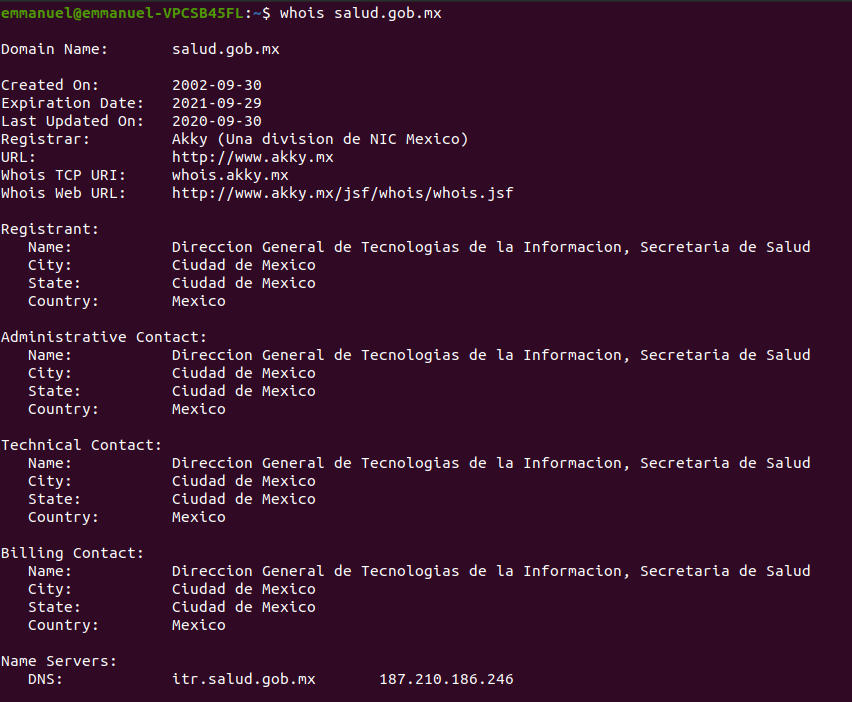
\includegraphics[width=\linewidth]{imagenes/whois_ss}

\section{nslookup}

El comando \texttt{nslookup} se usa para encontrar la dirección IP de un dominio. También se puede usar para encontrar el dominio de una dirección IP.

Se buscó información del dominio \texttt{pemex.com}. La dirección IP se puede ver en internet address.

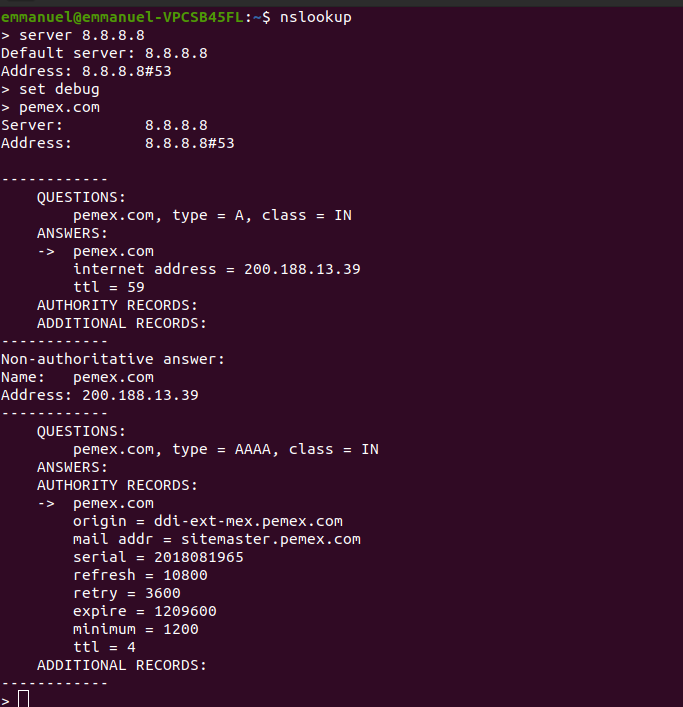
\includegraphics[width=\linewidth]{imagenes/nslookup_pemex}

\section{traceroute}

El comando \texttt{traceroute} determina la ruta tomada desde mi computadora hasta un host en el internet. Se muestran los routers por los que pasa un paquete antes de llegar a su destino. También se muestra el tiempo que tarda en pasar de un punto a otro.

Se buscó la dirección IP de \texttt{unam.mx} con \texttt{lookup}. Uno de los resultados es \texttt{132.248.166.20}.

Se realizó un trazado de ruta hacia la dirección IP de la UNAM.

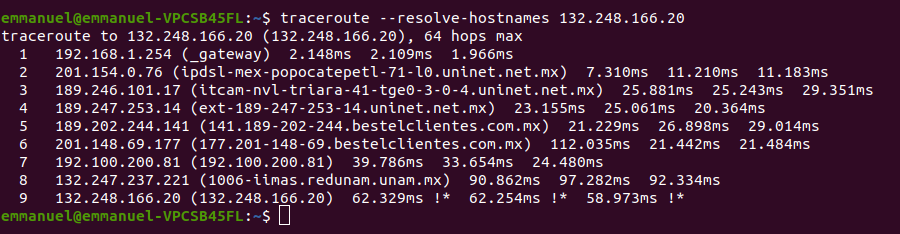
\includegraphics[width=\linewidth]{imagenes/traceroute_unam}

\section{nmap}

Nmap es una herramienta que se usa para determinar los hosts que se están ejecutando y los servicios que estos están ejecutando.

\subsection{Escaneo de puertos TCP}

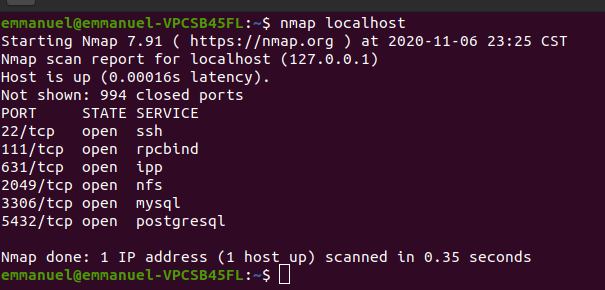
\includegraphics[width=\linewidth]{imagenes/puertos}

\subsection{Sistema operativo}

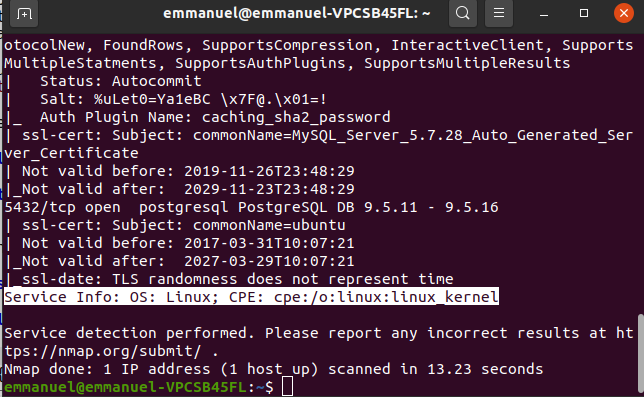
\includegraphics[width=\linewidth]{imagenes/sistema_operativo}


\end{document}

